\documentclass[a4paper,11pt]{article}

% === Packages ===
\usepackage[utf8]{inputenc}
\usepackage[T1]{fontenc}
\usepackage[french]{babel}
\usepackage{amsmath,amssymb}
\usepackage{graphicx}
\usepackage{booktabs}
\usepackage{hyperref}
\usepackage{geometry}
\usepackage{float}
\usepackage{caption}
\usepackage{subcaption}
\usepackage{listings}
\usepackage{xcolor}
\usepackage{multirow}
\usepackage{array}

\geometry{margin=2.5cm}

\lstset{
  basicstyle=\ttfamily\small,
  backgroundcolor=\color{gray!10},
  frame=single,
  breaklines=true,
  language=Python,
  keywordstyle=\color{blue},
  commentstyle=\color{green!50!black},
  stringstyle=\color{red!70!black},
}

% === Titre ===
\title{
  \textbf{Projet Module Deep Learning} \\[0.5em]
  \Large Herbiers \& CrossViT : Segmentation, pondération par patch et interprétabilité
}
\author{Roméo}
\date{2025--2026}

\begin{document}

\maketitle
\tableofcontents
\newpage

% ============================================================
\section{Introduction}

Ce rapport présente les travaux réalisés dans le cadre du projet de Deep Learning portant sur l'identification de spécimens d'herbiers numérisés. L'objectif principal est d'analyser l'impact de la segmentation sur l'apprentissage avec une architecture de type CrossViT (deux branches) et d'introduire une pondération par patch basée sur la densité de plante.

Le projet couvre cinq objectifs~:
\begin{enumerate}
  \item Comparaison de quatre configurations CrossViT (A, B, C1, C2)~;
  \item Modification de l'architecture pour deux branches de même résolution~;
  \item Pondération par patch et perte pondérée~;
  \item Interprétabilité via attention rollout, heatmaps et IoU~;
  \item Entraînement avec fonction de perte intégrant le terme IoU.
\end{enumerate}

La tâche de classification est binaire~: \textbf{présence} ou \textbf{absence d'épines} sur les spécimens.

% ============================================================
\section{Données et protocole expérimental}

\subsection{Jeu de données}

Le jeu de données est constitué de \textbf{898 paires d'images} alignées d'herbiers numérisés~:
\begin{itemize}
  \item \textbf{Image non segmentée}~: planche complète avec étiquettes, codes-barres et règles~;
  \item \textbf{Image segmentée}~: fond supprimé (noir), ne laissant que la plante.
\end{itemize}

Les étiquettes cibles sont binaires~: présence (1) ou absence (0) d'épines.

Un masque binaire est dérivé de l'image segmentée par seuillage ($>10$ sur le canal gris), ce qui permet d'identifier les pixels plante pour la pondération par patch et le calcul d'IoU.

\subsection{Protocole}

\begin{itemize}
  \item \textbf{Split}~: 80\% entraînement (718 images) / 20\% validation (180 images), reproductible (seed = 42).
  \item \textbf{Augmentations} (train)~: resize + random crop, flips horizontal/vertical, color jitter, rotation ($\pm 30°$), random grayscale (10\%), random erasing (20\%).
  \item \textbf{Normalisation}~: ImageNet (mean = [0.485, 0.456, 0.406], std = [0.229, 0.224, 0.225]).
  \item \textbf{Optimiseur}~: AdamW, $\text{lr} = 5 \times 10^{-5}$, weight decay = 0.05.
  \item \textbf{Scheduler}~: Cosine annealing ($\eta_{\min} = 10^{-6}$).
  \item \textbf{Époques}~: 5 (Partie~1) à 5 (Parties~2--5), batch size = 32 (GPU CUDA).
  \item \textbf{Métriques}~: Accuracy, F1-score (binaire), matrice de confusion.
\end{itemize}

% ============================================================
\section{Partie 1 — CrossViT de base \& comparaisons}

\subsection{Architecture de référence}

Nous utilisons le CrossViT-small pré-entraîné sur ImageNet avec deux branches~:
\begin{itemize}
  \item \textbf{Branche Small}~: image $240 \times 240$, patches de $12 \times 12$, embedding dimension 192, 6 têtes d'attention~;
  \item \textbf{Branche Large}~: image $224 \times 224$, patches de $16 \times 16$, embedding dimension 384, 6 têtes d'attention.
\end{itemize}

Les deux branches sont reliées par des blocs de \textit{cross-attention} (fusion croisée). La classification finale est obtenue par la moyenne des logits des tokens \texttt{[CLS]} des deux branches, suivie d'une tête linéaire adaptée à 2 classes.

Le modèle totalise \textbf{26\,279\,428 paramètres entraînables}.

\subsection{Configurations évaluées}

Quatre configurations sont testées, en variant quelle image (non segmentée ou segmentée) est envoyée à quelle branche~:

\begin{table}[H]
\centering
\begin{tabular}{clll}
\toprule
\textbf{Config} & \textbf{Branche Small ($240 \times 240$)} & \textbf{Branche Large ($224 \times 224$)} \\
\midrule
A  & Non segmentée & Non segmentée \\
B  & Segmentée & Segmentée \\
C1 & Non segmentée & Segmentée \\
C2 & Segmentée & Non segmentée \\
\bottomrule
\end{tabular}
\caption{Configurations CrossViT de la Partie~1.}
\end{table}

\subsection{Résultats}

\begin{table}[H]
\centering
\begin{tabular}{lcccccc}
\toprule
\textbf{Config} & \textbf{Best Val Acc} & \textbf{Best Val F1} & \textbf{Matrice de confusion} \\
\midrule
A  & 0.9722 & 0.9751 & — (config A incomplète à l'époque~1) \\
B  & 0.9667 & 0.9694 & $\begin{pmatrix} 79 & 2 \\ 4 & 95 \end{pmatrix}$ \\
C1 & 0.9556 & 0.9592 & $\begin{pmatrix} 78 & 3 \\ 5 & 94 \end{pmatrix}$ \\
C2 & \textbf{0.9722} & \textbf{0.9751} & $\begin{pmatrix} 77 & 4 \\ 1 & 98 \end{pmatrix}$ \\
\bottomrule
\end{tabular}
\caption{Résultats de la Partie~1 sur le jeu de validation (5 époques).}
\label{tab:part1}
\end{table}

% === NOTE POUR LES FIGURES ===
% Décommentez et ajustez les chemins si les images existent dans results/
% \begin{figure}[H]
%   \centering
%   \includegraphics[width=0.8\textwidth]{results/part1_B_curves.png}
%   \caption{Courbes d'apprentissage — Configuration B.}
% \end{figure}

\subsection{Analyse}

Les quatre configurations atteignent des performances très élevées ($>95\%$ F1-score), ce qui s'explique par l'utilisation de poids pré-entraînés ImageNet.

Les configurations \textbf{A} et \textbf{C2} obtiennent les meilleurs F1-scores (0.9751). La configuration C2 (segmentée $\to$ Small, non segmentée $\to$ Large) est particulièrement intéressante~: elle ne produit qu'\textbf{une seule erreur} de type faux négatif (1 plante avec épines classée sans épines), contre 4 pour la configuration B.

La configuration B (images segmentées uniquement) montre que la suppression du fond aide déjà significativement. Les configurations mixtes C1 et C2 confirment l'intérêt de combiner les deux types d'images dans les branches du CrossViT.

% ============================================================
\section{Partie 2 — Deux branches de même résolution}

\subsection{Architecture modifiée}

Nous modifions le CrossViT pour que les deux branches aient la \textbf{même résolution}~:
\begin{itemize}
  \item \textbf{Image size}~: $224 \times 224$ pour les deux branches~;
  \item \textbf{Patch size}~: $16 \times 16$ (196 patches par image)~;
  \item \textbf{Embedding dimension}~: 256~;
  \item \textbf{Profondeur}~: 4 blocs Transformer par branche~;
  \item \textbf{Têtes d'attention}~: 8 par bloc~;
  \item \textbf{Cross-attention}~: tous les 2 blocs (2 modules de cross-attention).
\end{itemize}

\textbf{Branche~1} reçoit l'image non segmentée, \textbf{Branche~2} reçoit l'image segmentée. Les poids ne sont \textbf{pas partagés} entre les branches. La classification est la moyenne des logits des deux têtes.

Ce modèle totalise \textbf{7\,869\,956 paramètres entraînables} (environ 3,3$\times$ moins que le CrossViT pré-entraîné), et il est entraîné \textbf{from scratch} (sans pré-entraînement ImageNet).

\subsection{Résultats}

\begin{table}[H]
\centering
\begin{tabular}{lccc}
\toprule
\textbf{Expérience} & \textbf{Best Val Acc} & \textbf{Best Val F1} & \textbf{Matrice (dernière ép.)} \\
\midrule
Part2 — Same resolution & 0.8111 & 0.8317 & $\begin{pmatrix} 49 & 32 \\ 9 & 90 \end{pmatrix}$ \\
\bottomrule
\end{tabular}
\caption{Résultats de la Partie~2 (5 époques, from scratch).}
\label{tab:part2}
\end{table}

\subsection{Comparaison avec la Partie~1}

\begin{table}[H]
\centering
\begin{tabular}{lcc}
\toprule
\textbf{Expérience} & \textbf{Best Val Acc} & \textbf{Best Val F1} \\
\midrule
Part1 A (pré-entraîné) & 0.9722 & 0.9751 \\
Part1 B (pré-entraîné) & 0.9667 & 0.9694 \\
Part1 C1 (pré-entraîné) & 0.9556 & 0.9592 \\
Part1 C2 (pré-entraîné) & 0.9722 & 0.9751 \\
\midrule
Part2 — Same res (from scratch) & 0.8111 & 0.8317 \\
\bottomrule
\end{tabular}
\caption{Comparaison Partie~1 vs Partie~2.}
\end{table}

\subsection{Analyse}

L'écart de performance ($\sim$15 points de F1) entre la Partie~1 et la Partie~2 s'explique principalement par~:
\begin{enumerate}
  \item L'\textbf{absence de pré-entraînement ImageNet} en Partie~2, alors que la Partie~1 bénéficie de représentations visuelles riches déjà apprises~;
  \item Un modèle plus petit (7.9M vs 26.3M paramètres)~;
  \item Seulement 5 époques d'entraînement sur un petit dataset (898 images).
\end{enumerate}

La matrice de confusion révèle que le modèle Partie~2 produit beaucoup de faux positifs (32), indiquant une difficulté à classifier correctement les images sans épines.

% ============================================================
\section{Partie 3 — Pondération par patch \& perte pondérée}

\subsection{Méthode}

Pour chaque image segmentée, le masque binaire est découpé en patches alignés avec le ViT. Pour chaque patch $p$, on calcule~:
\[
r_p = \frac{\text{nombre de pixels plante}}{\text{nombre total de pixels du patch}} \in [0, 1]
\]

Le calcul est réalisé efficacement via un \texttt{avg\_pool2d} avec un kernel de taille \texttt{patch\_size}.

Trois fonctions de pondération $f(r_p) = w_p$ sont testées~:

\begin{enumerate}
  \item \textbf{Linéaire}~: $w_p = \varepsilon + r_p$ \quad avec $\varepsilon = 0.1$
  \item \textbf{Puissance}~: $w_p = (\varepsilon + r_p)^{\gamma}$ \quad avec $\gamma = 0.5$
  \item \textbf{Normalisée}~: $\tilde{w}_p = \frac{w_p}{\frac{1}{P}\sum_q w_q}$ \quad (moyenne unitaire par image)
\end{enumerate}

\textbf{Propagation}~: les mêmes poids $w_p$ sont assignés aux patches co-localisés de l'image non segmentée (même grille, même taille de patch, même alignement).

\textbf{Intégration}~: les poids sont multipliés aux embeddings des patch tokens après le positional embedding, avant les blocs Transformer. La perte est une CrossEntropy pondérée par le poids moyen des patches de chaque image.

\subsection{Résultats}

\begin{table}[H]
\centering
\begin{tabular}{lccc}
\toprule
\textbf{Fonction $f$} & \textbf{Best Val Acc} & \textbf{Best Val F1} & \textbf{Matrice (dernière ép.)} \\
\midrule
Sans pondération (Partie~2) & 0.8111 & 0.8317 & $\begin{pmatrix} 49 & 32 \\ 9 & 90 \end{pmatrix}$ \\
Linéaire ($\varepsilon + r_p$) & 0.8167 & 0.8436 & $\begin{pmatrix} 58 & 23 \\ 10 & 89 \end{pmatrix}$ \\
Puissance ($(\varepsilon + r_p)^{0.5}$) & \textbf{0.8500} & \textbf{0.8683} & $\begin{pmatrix} 64 & 17 \\ 10 & 89 \end{pmatrix}$ \\
Normalisée & 0.8333 & 0.8515 & $\begin{pmatrix} 59 & 22 \\ 12 & 87 \end{pmatrix}$ \\
\bottomrule
\end{tabular}
\caption{Comparaison des fonctions de pondération (Partie~3, 5 époques).}
\label{tab:part3}
\end{table}

\subsection{Analyse}

La pondération par patch améliore systématiquement les performances par rapport au modèle Partie~2 de base~:
\begin{itemize}
  \item La \textbf{pondération puissance} ($\gamma = 0.5$) obtient les meilleurs résultats (+3.66 points de F1), avec une nette réduction des faux positifs (de 32 à 17).
  \item L'exposant $\gamma = 0.5$ (racine carrée) amplifie la contribution des patches avec peu de plante, ce qui semble aider le modèle à mieux utiliser les zones marginales du spécimen.
  \item La normalisation (moyenne unitaire) aide également mais moins que la puissance, suggérant que le scaling absolu des poids est important.
\end{itemize}

% ============================================================
\section{Partie 4 — Heatmaps / Attention Rollout \& IoU}

\subsection{Méthode d'attention rollout}

L'\textit{attention rollout} agrège les matrices d'attention de toutes les couches pour estimer l'influence globale de chaque patch sur le token \texttt{[CLS]}~:
\begin{enumerate}
  \item Pour chaque couche $l$~: moyenne des têtes $A^{(l)}$
  \item Ajout de l'identité~: $A^{(l)} \leftarrow A^{(l)} + I$ (connexion résiduelle)
  \item Renormalisation des lignes~: $A^{(l)} \leftarrow A^{(l)} / \sum_j A^{(l)}_{ij}$
  \item Produit cumulatif~: $\tilde{A} = \prod_l A^{(l)}$
  \item Extraction~: attention du \texttt{[CLS]} vers chaque patch ($\tilde{A}[0, 1:]$)
\end{enumerate}

La carte obtenue est reshape en grille et interpolée à la taille de l'image pour produire la heatmap.

Pour le CrossViT multi-résolution (Partie~1), les attentions sont séparées par branche et seule la branche Large (196 patches) est utilisée pour la heatmap finale.

\subsection{Calcul de l'IoU}

La heatmap d'attention est binarisée au quantile 0.8, puis comparée au masque plante~:
\[
\text{IoU} = \frac{|M_{\text{att}} \cap M_{\text{plante}}|}{|M_{\text{att}} \cup M_{\text{plante}}|}
\]

\subsection{Résultats IoU sur la validation}

\begin{table}[H]
\centering
\begin{tabular}{lcc}
\toprule
\textbf{Modèle} & \textbf{IoU Moyen} & \textbf{Écart-type IoU} \\
\midrule
Partie~1 — Config A & 0.1456 & 0.1253 \\
Partie~1 — Config B & \textbf{0.4819} & 0.1308 \\
Partie~1 — Config C1 & 0.4594 & 0.1507 \\
Partie~1 — Config C2 & 0.2053 & 0.1357 \\
Partie~2 — Même résolution (baseline) & 0.1919 & 0.1673 \\
\bottomrule
\end{tabular}
\caption{IoU moyen (attention rollout vs masque plante) sur la validation.}
\label{tab:iou}
\end{table}

\subsection{Analyse des heatmaps}

\begin{itemize}
  \item \textbf{Config B} (images segmentées uniquement) obtient le meilleur IoU (0.48), ce qui est cohérent~: le modèle n'a accès qu'à la plante, donc son attention se concentre naturellement sur les régions végétales.
  \item \textbf{Config A} (non segmentées uniquement) a le plus faible IoU (0.15), indiquant que le modèle utilise fortement les éléments d'arrière-plan (étiquettes, codes-barres) pour classifier.
  \item \textbf{Config C1} a un bon IoU (0.46) grâce à la branche Large qui reçoit l'image segmentée.
  \item \textbf{Config C2} a un IoU plus faible (0.21) car l'attention rollout est extraite de la branche Large qui reçoit l'image non segmentée.
  \item Le modèle \textbf{Partie~2} (from scratch) a un IoU faible (0.19), cohérent avec un modèle non pré-entraîné qui n'a pas encore appris à se focaliser sur les régions pertinentes.
\end{itemize}

% Décommentez si les figures existent :
% \begin{figure}[H]
%   \centering
%   \includegraphics[width=0.9\textwidth]{results/part4_heatmap_examples.png}
%   \caption{Exemples de heatmaps d'attention pour chaque modèle.}
% \end{figure}
%
% \begin{figure}[H]
%   \centering
%   \includegraphics[width=0.7\textwidth]{results/part4_iou_comparison.png}
%   \caption{Comparaison des IoU moyens par configuration.}
% \end{figure}

% ============================================================
\section{Partie 5 — Entraînement avec perte IoU}

\subsection{Fonction de perte}

Pour forcer le modèle à focaliser son attention sur la plante, nous intégrons l'IoU dans la fonction de perte~:
\[
\mathcal{L}_{\text{total}} = \mathcal{L}_{\text{CE}} + \lambda \cdot \mathcal{L}_{\text{IoU}}
\]

avec $\mathcal{L}_{\text{IoU}} = 1 - \text{mean}(\text{IoU}_{\text{soft}})$ et $\lambda = 1.0$.


\subsection{Résultats}

\begin{table}[H]
\centering
\begin{tabular}{lccc}
\toprule
\textbf{Modèle} & \textbf{Best Val F1} & \textbf{IoU Moyen} & \textbf{Amélioration IoU} \\
\midrule
Part2 — Sans IoU loss & 0.8317 & 0.1919 & — \\
Part2 — Avec IoU loss ($\lambda=1$) & 0.8241 & \textbf{0.5061} & +163.8\% \\
\bottomrule
\end{tabular}
\caption{Impact de la loss IoU sur les performances et l'interprétabilité.}
\label{tab:part5}
\end{table}

Détail de l'entraînement avec loss IoU (5 époques)~:

\begin{table}[H]
\centering
\small
\begin{tabular}{ccccccc}
\toprule
\textbf{Époque} & \textbf{Train Loss} & \textbf{Train Acc} & \textbf{Train F1} & \textbf{Val Loss} & \textbf{Val Acc} & \textbf{Val F1} \\
\midrule
1 & 1.4800 & 0.6017 & 0.6603 & 0.5704 & 0.7667 & 0.8073 \\
2 & 1.4464 & 0.6156 & 0.6714 & 0.5485 & 0.7889 & 0.8241 \\
3 & 1.3987 & 0.6574 & 0.6830 & 0.5880 & 0.6167 & 0.7273 \\
4 & 1.3636 & 0.6783 & 0.7240 & 0.6264 & 0.6111 & 0.7266 \\
5 & 1.3569 & 0.6741 & 0.7167 & 0.5107 & 0.7611 & 0.8089 \\
\bottomrule
\end{tabular}
\caption{Détail de l'entraînement Partie~5 (loss CE + IoU).}
\end{table}

La décomposition de la loss montre que le terme CE diminue (de 0.6931 à 0.5961) tandis que le terme IoU diminue aussi (de 0.7870 à 0.7608), indiquant que le modèle apprend progressivement à focaliser son attention sur la plante.

\subsection{Comparaison des heatmaps : sans vs avec loss IoU}

La comparaison quantitative sur l'ensemble de validation montre une amélioration spectaculaire de l'IoU~:

\begin{table}[H]
\centering
\begin{tabular}{lccc}
\toprule
& \textbf{Moyenne IoU} & \textbf{Médiane IoU} & \textbf{Écart-type} \\
\midrule
SANS IoU loss & 0.1919 & 0.1446 & 0.1673 \\
AVEC IoU loss & 0.5061 & 0.5239 & 0.1330 \\
\midrule
\textbf{Amélioration} & \textbf{+0.3143} & \textbf{+0.3793} & — \\
\bottomrule
\end{tabular}
\caption{Comparaison IoU : sans vs avec régularisation IoU.}
\end{table}

% Décommentez si les figures existent :
% \begin{figure}[H]
%   \centering
%   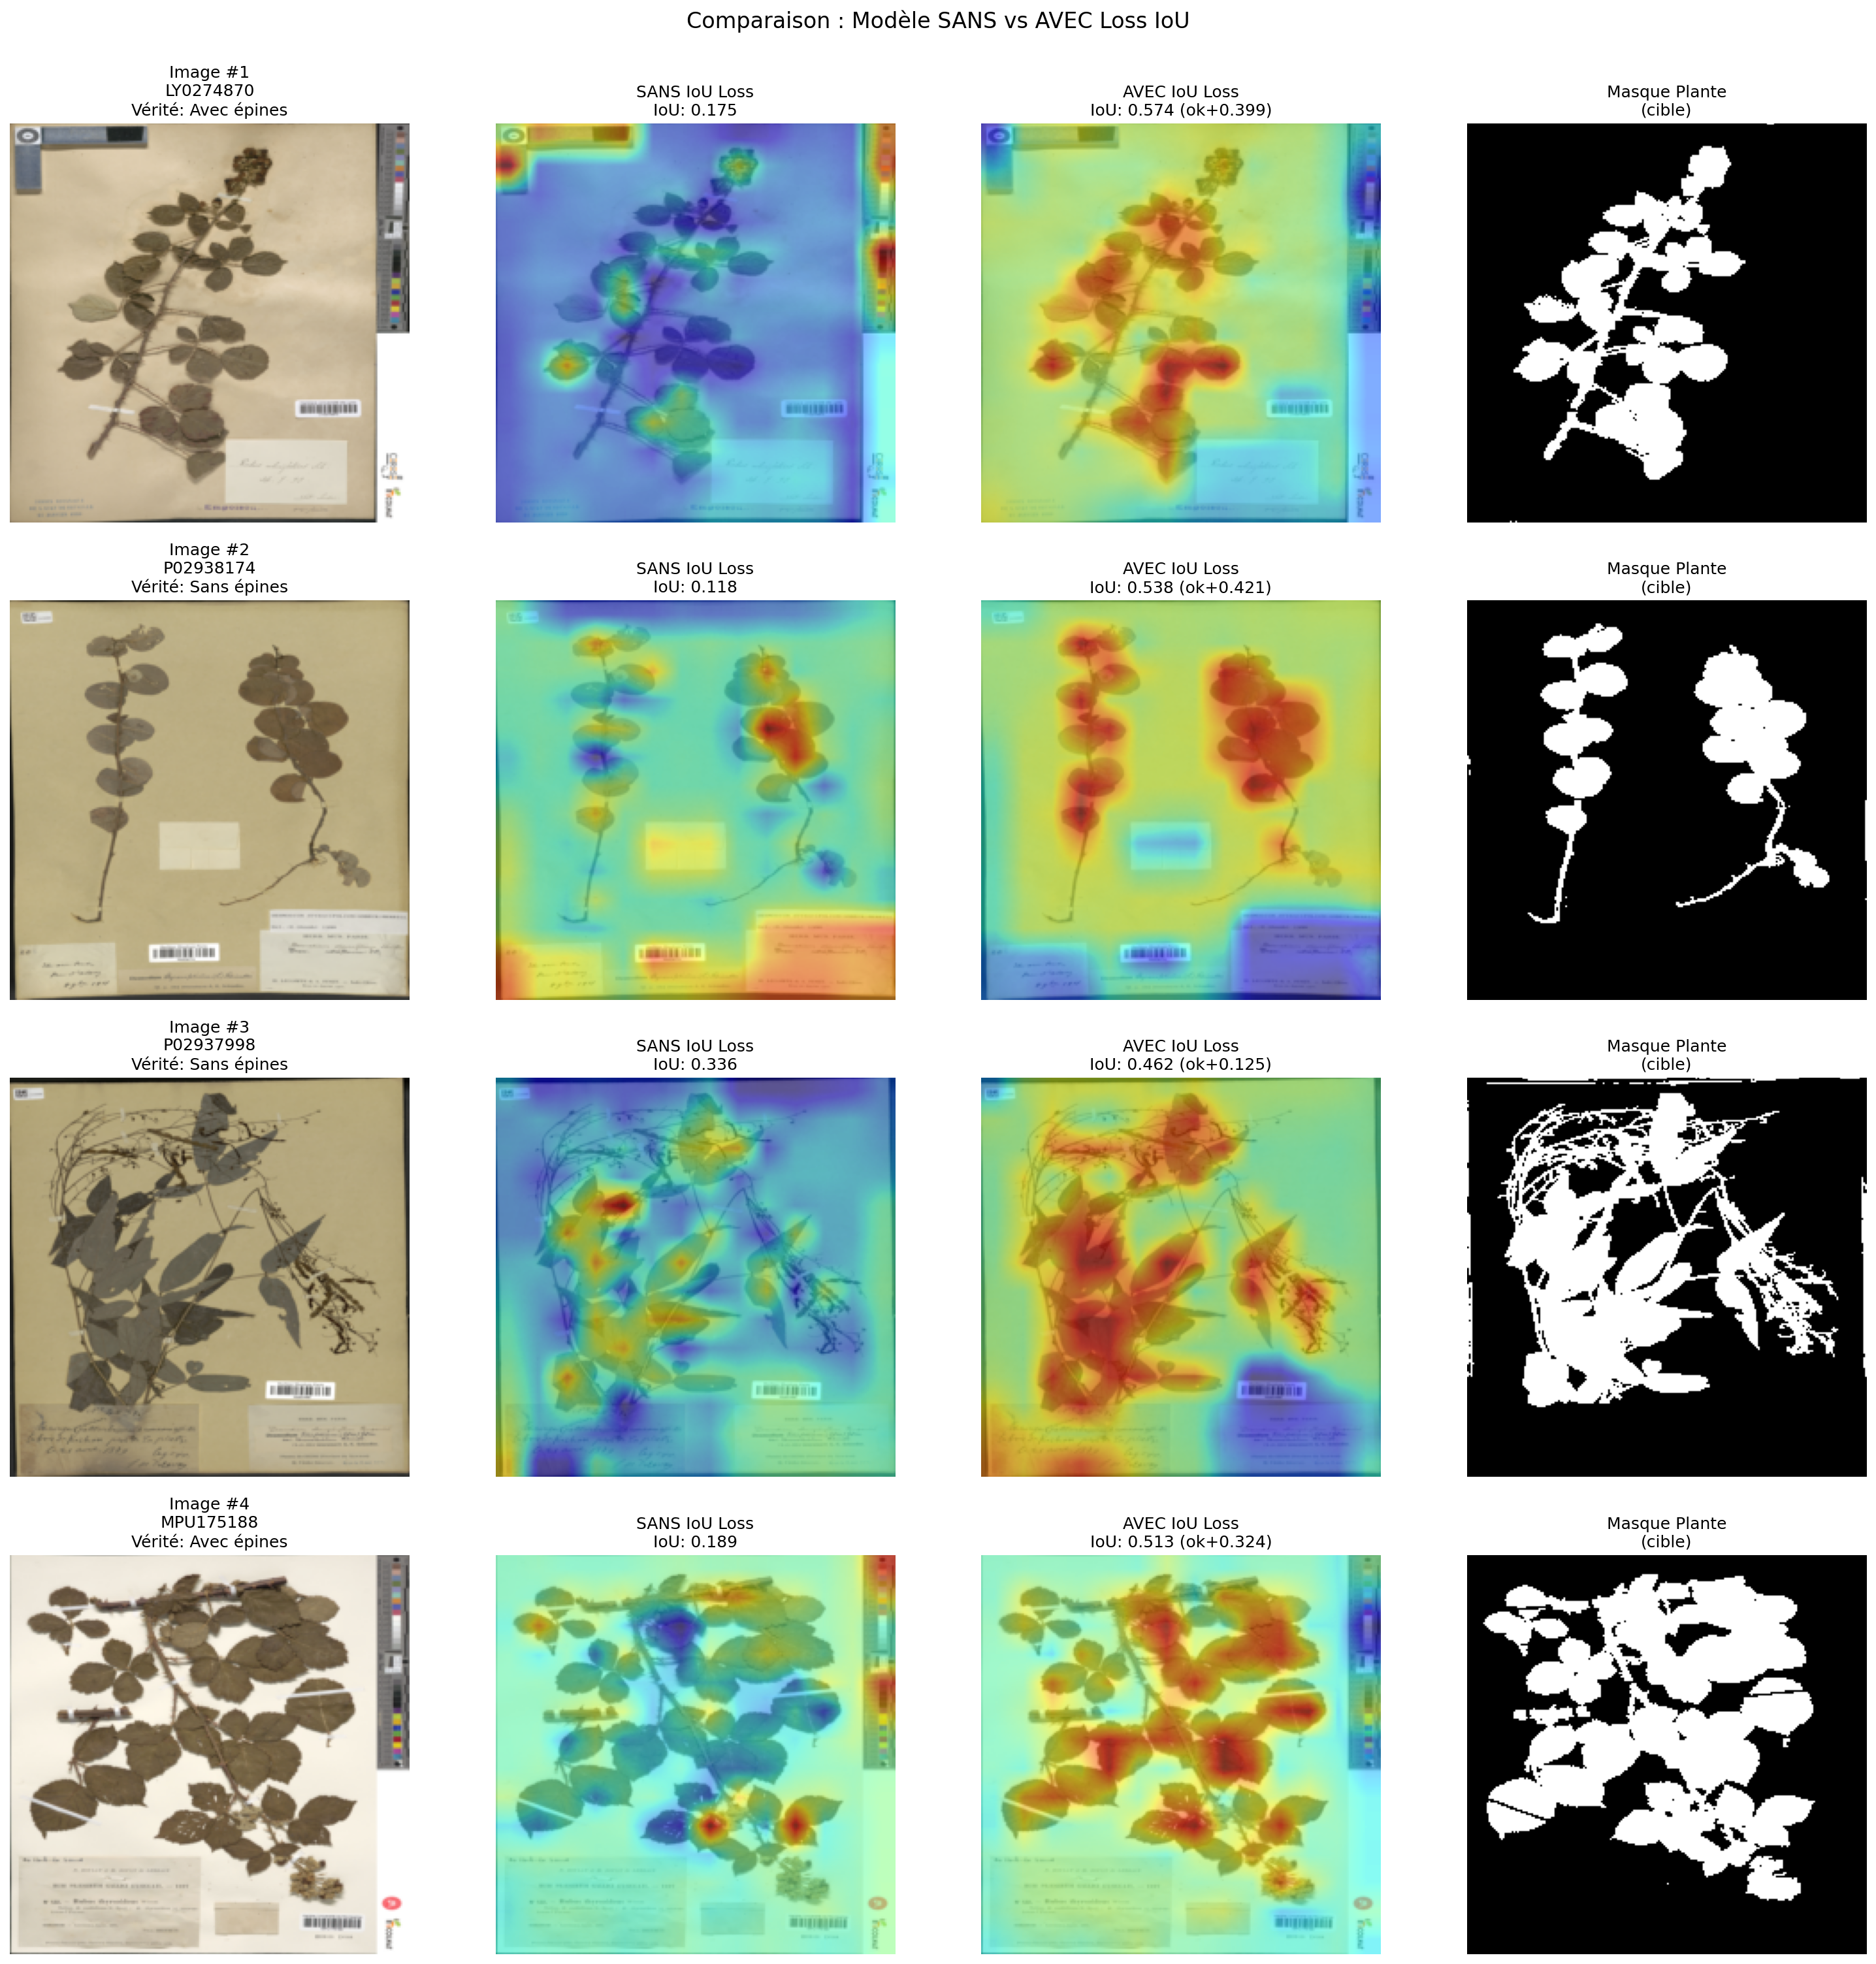
\includegraphics[width=0.8\textwidth]{results/part4_comparison_baseline_vs_iou.png}
%   \caption{Comparaison visuelle des heatmaps SANS vs AVEC loss IoU.}
% \end{figure}
%
% \begin{figure}[H]
%   \centering
%   \includegraphics[width=0.7\textwidth]{results/part4_iou_comparison_distribution.png}
%   \caption{Distribution des IoU : SANS vs AVEC loss IoU.}
% \end{figure}

\subsection{Analyse}

L'intégration de l'IoU dans la perte produit une \textbf{amélioration significative} de l'interprétabilité (+163.8\% d'IoU en moyenne). Le modèle apprend à concentrer son attention sur les régions de la plante plutôt que sur l'arrière-plan.

En termes de performance de classification, le F1-score diminue très légèrement (0.8317 $\to$ 0.8241, soit $-$0.9\%), ce qui constitue un compromis acceptable entre performance et interprétabilité. Cette légère baisse peut s'expliquer par le fait que certaines informations contextuelles de l'arrière-plan (étiquettes, position) étaient utilisées par le modèle baseline pour la classification.

% ============================================================
\section{Tableau récapitulatif global}

\begin{table}[H]
\centering
\small
\begin{tabular}{llccc}
\toprule
\textbf{Partie} & \textbf{Expérience} & \textbf{Best Val Acc} & \textbf{Best Val F1} & \textbf{IoU Moyen} \\
\midrule
\multirow{4}{*}{1 (pré-entraîné)}
& Config A & 0.9722 & 0.9751 & 0.146 \\
& Config B & 0.9667 & 0.9694 & 0.482 \\
& Config C1 & 0.9556 & 0.9592 & 0.459 \\
& Config C2 & 0.9722 & \textbf{0.9751} & 0.205 \\
\midrule
2 (from scratch) & Same resolution & 0.8111 & 0.8317 & 0.192 \\
\midrule
\multirow{3}{*}{3 (pondération)}
& Linéaire & 0.8167 & 0.8436 & — \\
& Puissance ($\gamma\!=\!0.5$) & 0.8500 & 0.8683 & — \\
& Normalisée & 0.8333 & 0.8515 & — \\
\midrule
5 (loss IoU) & Same res + IoU & 0.7889 & 0.8241 & 0.506 \\
\bottomrule
\end{tabular}
\caption{Tableau récapitulatif de toutes les expériences.}
\label{tab:global}
\end{table}

% ============================================================
\section{Architecture du code}

Le projet est organisé en modules Python réutilisables~:

\begin{table}[H]
\centering
\begin{tabular}{ll}
\toprule
\textbf{Fichier} & \textbf{Rôle} \\
\midrule
\texttt{config.py} & Configuration centralisée (chemins, hyperparamètres) \\
\texttt{dataloader.py} & Dataset PyTorch + augmentations + split train/val \\
\texttt{model.py} & CrossViT Partie~1 (wrapper A/B/C1/C2) \\
\texttt{model\_same\_res.py} & CrossViT Partie~2 (même résolution) \\
\texttt{patch\_weights.py} & Calcul des poids par patch (Partie~3) \\
\texttt{attention\_rollout.py} & Hooks, rollout, IoU, loss IoU (Parties~4--5) \\
\texttt{train.py} & Script d'entraînement unifié \\
\texttt{evaluate.py} & Évaluation, heatmaps, comparaison \\
\texttt{notebook\_part*.ipynb} & Notebooks d'exécution et visualisation \\
\bottomrule
\end{tabular}
\caption{Structure du code source.}
\end{table}

% ============================================================
\section{Discussion et conclusion}

\subsection{Principaux résultats}

\begin{enumerate}
  \item \textbf{Le pré-entraînement ImageNet domine}~: les configurations Partie~1 (F1 $>$ 0.95) surpassent largement la Partie~2 (F1 $\approx$ 0.83), confirmant l'importance du transfer learning sur un petit jeu de données.

  \item \textbf{La segmentation aide mais n'est pas indispensable}~: la Config~A (non segmentée uniquement) rivalise avec la Config~B (segmentée uniquement), voire la surpasse légèrement, car le modèle pré-entraîné peut exploiter le contexte global.

  \item \textbf{La pondération par patch améliore le modèle from scratch}~: la fonction puissance ($\gamma = 0.5$) apporte +3.66 points de F1, montrant que guider l'attention vers les régions de plante est bénéfique.

  \item \textbf{La loss IoU améliore massivement l'interprétabilité}~: l'IoU passe de 0.19 à 0.51 (+164\%), avec un coût négligeable en performance ($-$0.9\% F1). Le modèle apprend à regarder la plante plutôt que l'arrière-plan.
\end{enumerate}

\subsection{Limites}

\begin{itemize}
  \item Le nombre d'époques est limité (5) pour la plupart des expériences, ce qui ne permet pas au modèle from scratch d'atteindre son plein potentiel.
  \item Le jeu de données est petit (898 images), ce qui rend le modèle sensible au split et aux augmentations.
  \item L'attention rollout pour le CrossViT multi-résolution ne prend que la branche Large, ce qui peut sous-estimer l'attention de la branche Small.
\end{itemize}

\subsection{Perspectives}

\begin{itemize}
  \item Augmenter le nombre d'époques et combiner pondération par patch + loss IoU.
  \item Explorer d'autres architectures (ViT standard, DeiT) pour comparaison.
  \item Utiliser un vrai masque de segmentation au lieu du seuillage simple.
  \item Tester la pondération par patch sur le modèle pré-entraîné (Partie~1).
\end{itemize}

\end{document}
